% !Mode:: "TeX:UTF-8"
\definecolor{dkgreen}{rgb}{0,0.6,0}
\definecolor{gray}{rgb}{0.5,0.5,0.5}
\definecolor{mauve}{rgb}{0.58,0,0.82}

\lstset{frame=tb,
  language=Mathematica,
  aboveskip=3mm,
  belowskip=3mm,
  showstringspaces=false,
  columns=flexible,
  basicstyle={\small\ttfamily},
  numbers=left,
  numberstyle=\tiny\color{gray},
  keywordstyle=\color{blue},
  commentstyle=\color{dkgreen},
  stringstyle=\color{mauve},
  breaklines=true,
  breakatwhitespace=true
  tabsize=3
}
\chapter{ss方程守恒律程序包开发}
第二章第二节中介绍了偏微分方程的守恒律,守恒律作为非线性偏微分方程中一个很重要的性质,对于研究非线性偏微分来说具有很重要的作用。然而,求解偏微分方程守恒律的过程并不是一成不变的,一般来说不同类型方程的求解方式会具有很大的差异,在求解的过程中,往往只能凭借研究人员的个人的思考和过往研究经验对中间过程进行人工处理,才能得到最终的结果。幸运的是,在求解方程守恒律的过程中并不是所有的步骤都需要人工式的处理,仍然有一些步骤是机械式的流程,对于不同类型的方程,只要给出足够必要的条件,就能不断的迭代产生出从第一项到任意一项的守恒律。以 Sasa-Satsuma 方程为例,首先得到目标方程分别关于时间和空间多项式 $D_n$ 和 $F_n$ 的表达式,然后再得到表达式中依赖项的形式和起始项,就很容易的可以推导出任意一项的守恒律,最后进行验证是否正确。 因此可以将这一部分流程抽象出来,编写出用于求解守恒律的程序包。本章将主要介绍使用 Mathematica 内置的编程语言 Wolfram 来封装求解守恒律过程的程序包。

\section{Mathematica 基本介绍}
Wolfram 语言主要用于解决符号计算和函数式编程,它的语法和用法与其它高级语言有很大不同。Wolfram 语言是交互式语言,在 Mathematica 编辑器中敲入输入,然后按下 Shift+Enter 便可运行输出结果,另一种情况是在输入后添加分号,按下 Shift+Enter 则只计算但不输出计算结果。相比于 C 语言和其他面向对象语言,Wolfram 语言的语法规则十分简单。Wolfram 中的一切都是符号表达式,没有元素类型的划分。而符号表达式主要分为两类,第一类是原子表达式:数字、实数、分数、复数、符号和字符串等;而由原子表达式组成的普通表达式一般都具有相同的基本结构:$head[arguments]$

${1,2,3} \cdots List[1,2,3]$

$1+2 \cdots Plus[1,2]$\\
其中 $head$ 成为头部,$arguments$ 是该表达式的参数,参数也可以是符号表达式:

$x^2+2y^2 \cdots Plus[Power[x,2],Times[2,Power[y,2]]]$

\begin{itemize}
\item 列表
\end{itemize}

列表是 Wolfram 语言的一种最常见的存储变量的数据结构,可以存储任意类型和任意容量的数据的集合,类似于其它语言的数组或者序列。列表在 Wolfram 中用 ${\cdots}$ 表示,列表中的元素可以是任何类型的表达式,列表的索引从 1 开始,可以用 $[[\cdots]]$ 提取列表的元素:

${a,b,c}[[1]]$ 的结果是 $a$.
\begin{itemize}
\item 函数
\end{itemize}

下列是定义一个带有 $x$ 和 $y$ 两个参数的函数

$f[\_x,\_y]:= x+y$

使用上面定义的函数:

$f[1,2]$ 的结果是 3.

一般来说,在一个自定义的函数中会用到其他辅助变量,但是 Wolfram 语言默认定义的变量是全局变量,当定义多个函数时需要注意同名变量相互覆盖的问题,为解决这个问题,Wolfram 提供 Module 模块定义局部变量:

$f[\_x,\_y]:=(Module[{a,b},\cdots])$

其中 $a,b$ 是局部变量,省略号处为函数体。另外,函数表达式还可以使用 /; 限制定义,使其只适用于某种条件:

$f[\_x,\_y]:= x-y/;x>y$

Wolfram 语言除了自定义函数,还有近 5000 个内置函数,前面介绍的列表是 Wolfram 语言中最常用的数据结构,下面给出一些 Wolfram 语言内置的关于列表操作的函数:

$Prepend[list,element]$	\quad 在 list 的开头添加元素 element

$Append[list,element]$	\quad 在 list 的末尾添加元素 element

$Insert[list,element,i]$ \quad	在 list 的第 i 个位置上插入 element

$Insert[list,element,-i]$ \quad	在 list 的倒数第 i 个位置上插入 element\\
另外还有一些常用的内置函数

$Expand[exp]$ \quad                       展开表达式 $exp$ 的每一项

$Simplify[exp]$  \quad                     化简表达式 $exp$

$Solve[eq,x]$  \quad           解关于未知数 $x$ 的方程 $eq$

$NSolve[\{eql,eq2,...\},\{x1, x2...\}]$   \quad    解关于未知数 $xi$ 的方程组 $eq1,eq2,...$

$D[f,x]$     \quad                    关于函数 $f$ 对 $x$ 求微分

$D[f,{x,n}]$     \quad                    关于函数 $f$ 求 $x$ 的 $n$ 次微分

$Coefficient[exp,item]$   \quad       取多项式 exp 中 item 项的系数
\section{变量变换方法的实现}
如果已知一个简单方程的怪波解,那么我们就可以求得同类型复杂方程的怪波解,首先要求得复杂方程到简单方程的关系表达式。\\

以下是实现代码:
\begin{lstlisting}[language=Mathematica,caption=变量变换方法的实现]
(*coe1第一个方程的各项系数组成的列表*)
(*coe2第二个方程的各项系数组成的列表*)
(*item1两个方程各项的函数部分组成的列表*)
(*item2第一个方程的项变量替换后的项的形式*)

DeReplace[coe1_,coe2_,item1_,item2_]:=(Module[{equ1,equ2,coe3,constrants,i,j,k},
equ1=0;
equ2=0;
coe3=List[];
constrants=List[];
For[i=1,i<Length[coe1]+1,i++,
equ1=equ1+coe1[[i]]*item1[[i]];
];

u^{(1,0)}[x,t]=D[u[x,t],x];
u^{(0,1)}[x,t]=D[u[x,t],t];
v^{(1,0)}[x,t]=D[v[x,t],x];
u^{(2,0)}[x,t]=D[u[x,t],{x,2}];
u^{(3,0)}[x,t]=D[u[x,t],{x,3}];
u[x,t]=A U[X[x,t],T[t]];
v[x,t]=A V[X[x,t],T[t]];
X[x,t]=a x + b ;
a2[t]=m a5[t];
equ3=Expand[equ1];
For[j=1,j<Length[item2]+1,j++,
coe3=Append[coe3,Coefficient[equ3,item2[[j]]]];
]

Print["变量变换后的系数:"];
Print[coe3];
flag=coe3[[1]]/coe2[[1]];
For[k=2,k<Length[coe2]+1,k++,
constrants=Append[constrants,coe3[[k]]==coe2[[k]]*flag]
]
Print["约束条件:"];
Print[constrants];
NSolve[constrants,{Derivative[1][T][t],A,a,b}]
])
\end{lstlisting}
$DeReplace$ 函数接收四个参数,$coe1$ 是复杂方程的各项系数组成的列表,$coe2$ 是简单方程的各项系数组成的列表,$item1$ 是复杂方程各项的函数部分组成的列表,因为复杂方程与简单方程同类型,所以有相同的项,$item2$ 是变量变换后的各项的函数部分组成的列表。首先通过循环将 $coe1$ 和 $item1$ 还原简单方程表达式赋值给 $equ1$,然后假设变量变换的表达式为
\begin{align}
&u[x,t]=A U[X[x,t],T[t]],\label{wol-1}\\
&v[x,t]=A V[X[x,t],T[t]],\\
&X[x,t]=a x + b. \label{wol-2}
\end{align}
$a2[t]=m a5[t]$ 是 Painlev\'{e} 可积条件,将式 (\ref{wol-1})-(\ref{wol-2}) 代入 $equ1$ 便得到变量变换后的方程表达式 $equ3$,获取 $equ3$ 各项的系数存入列表 $coe3$,然后找出新的系数列表 $coe3$ 与简单方程的系数列表 $coe2$ 之间的约束关系列表 $constrants$,最后通过解方程组求出 $T[t], a, b, A$ 的值,也就得到了前面假设的变量变换关系。

以简单方程 (\ref{ss-9}) 和复杂方程 (\ref{ss-1}) 为例,运用上述函数求得方程 (\ref{ss-9}) 和方程 (\ref{ss-1}) 的变量变换关系表达式:
\begin{figure}[!htp]
\centering
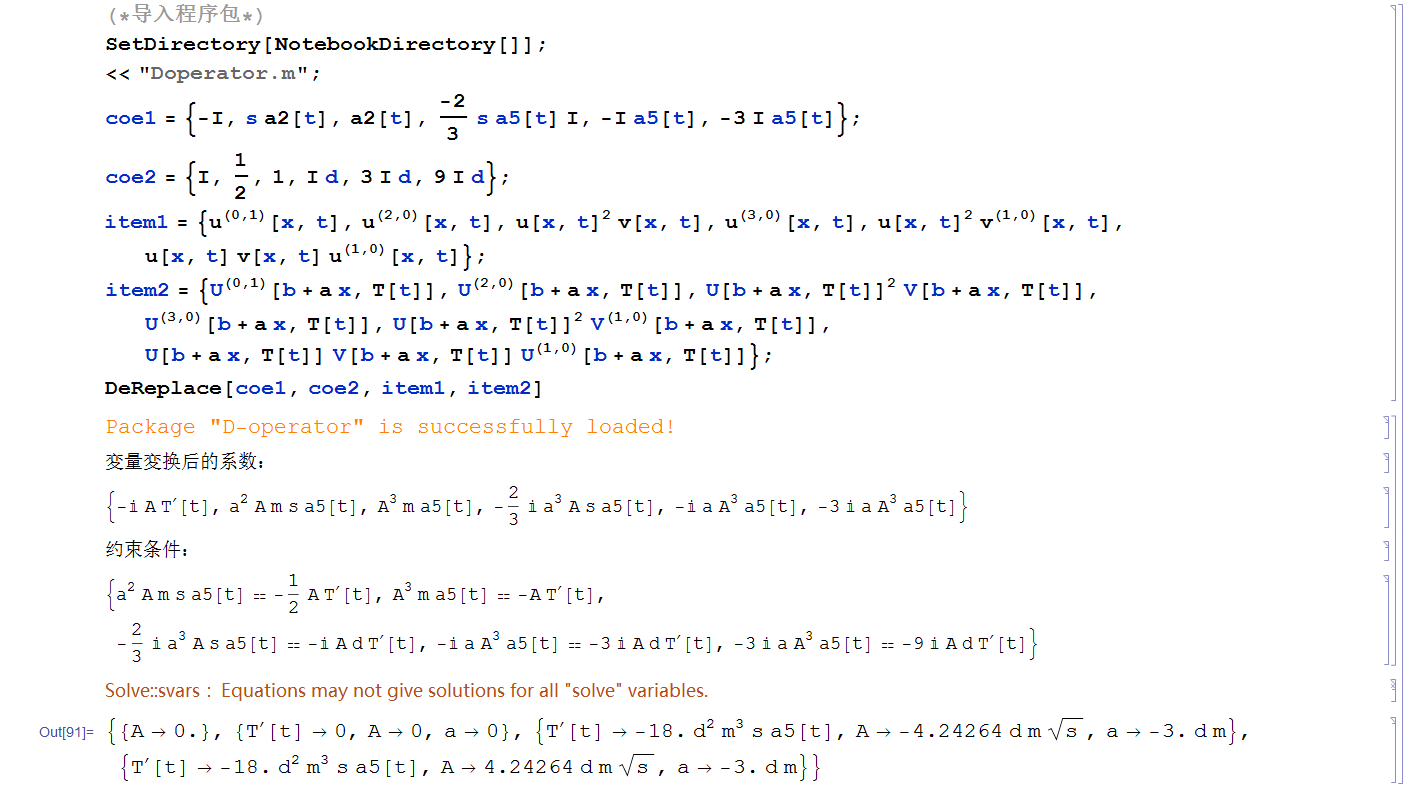
\includegraphics[width=\linewidth]{replaceResult.jpg}
\caption{变量变换运行结果}
%with same parameters~$k=1 , \alpha_2(t)=1, \alpha_0(t)=0$.
\label{pro-doper3}
\end{figure}
为调用 $DeReplace$ 函数,首先要导入封装该函数的程序包 $Doperator.m$,Mathematica 提供的自定义程序包是以 .m 为后缀的文件。$Package "D-operator" is successfully loaded!$ 是程序包成功加载的自定义输出,运行结果打印出这句话,说明程序包成功加载。从输入可以看到,$coe1$ 和 $item1$ 分别是方程 (\ref{ss-1}) 的系数列表和项的函数列表,$coe2$ 和 $item1$ 分别是方程 (\ref{ss-9}) 的系数列表和项的函数列表,$item2$ 是方程 (\ref{ss-1}) 变量变换后项的函数列表,调用 $DeReplace$ 函数可以看到打印出的一系列中间结果和最后的输出结果。由假设的变量变换形式 (\ref{wol-1})-(\ref{wol-2}) 可以看出我们需要求解 $T[t], a, b, A$ 四个未知变量,将约束条件中的五个等式解方程组得到了最后输出结果的四组解。显然,$A$ 和 $a$ 不能为零,所以只有后两组解是我们想要的结果。还可以注意到,后两组解中都没有给出变量 $b$ 的表达式,也就是说 $b$ 是自由的,可以取任意值。至此我们得到了方程 (\ref{ss-9}) 和方程 (\ref{ss-1}) 的变量变换关系表达式 (\ref{wol-1})-(\ref{wol-2}),其中
\begin{align}
 &T[t]=-18 d^2 s m^3 \int a5[t] dt + C,\nonumber\\
 &X[x,t]=-3 d m x,\nonumber\\
 &A = \pm 3 \sqrt{2} d m \sqrt{s}.\nonumber
\end{align}
$C$ 为任意积分常数。

\section{验证怪波解}
上一节实现了两个方程的变量变换,接下来将变量变换关系应用于方程的已知怪波解,就能得到另一个方程的怪波解,并且进行验证。具体实现代码如下:

\begin{lstlisting}[language=Mathematica,caption=验证怪波解]
(*将第一个方程到第二个方程的变量变换的结果应用到第二个方程的怪波解上可以得到第一个方程的怪波解*)
(*X T A 分别是前一步变量变换求得的结果*)
(*equ第一个方程,即最后我们要验证怪波解的方程*)
DeRogue[X_,T_,A_,equ_]:=(Module[{d,c,k},
d=1;
c=1;
k=1;
a2[t]=m a5[t];
K=1+3k;
u0[x,t]=-A c/(2d) Exp[-I/(2d) (k X-w/(4d) T)];
v0[x,t]=-A c/(2d) Exp[I/(2d) (k X-w/(4d) T)];
w=2c^2 (1+3k)-k^2-k^3;
G=(d^2 (9c^2+2K^2))/(2c^2 K^2) (a+(4k1^2 k2^2)/(9c^2+2K^2) T)^2+(8d^2 k1^2 k2^2 (k1^2-k2^2))/(c^2 (9c^2+2K^2)) T^2+(162d^6 (9c^2+2K^2)^3)/(c^2 k1^2 k2^2 (k1^2+k2^2)^2);
H=1/(2K) (a^2/4+k1^2 k2^2 T^2-(243d^4 (9c^2+2K^2)^2)/(k1^2 k2^2 (18c^2+K^2)))(a+(4k1^2 k2^2)/(9c^2) T)+(16d^4 k1^2 k2^2 (27c^2+2K^2))/(c^4 K(18c^2+K^2)) T;
B=1/(36d^2) (a^2/4+k1^2 k2^2 T^2+(18^2 d^4 (k1^4-k1^2 k2^2-k2^4))/(k1^2 k2^2 (k1^2+k2^2)))^2+(9d^2 k2^2)/(k1^2+k2^2)^2 (a+2k1^2 T)^2+(108^2 d^6)/(k2^2 (k1^2+k2^2));
a=(K^2-1-27c^2)T+12d X;
k1=Sqrt[2]/2 (Sqrt[K^2 (18c^2+K^2)]-9c^2+K^2)^(1/2);
k2=Sqrt[2]/2 (Sqrt[K^2 (18c^2+K^2)]+9c^2-K^2)^(1/2);
u[x,t]=u0[x,t](1-(G+I H)/B);
v[x,t]=v0[x,t](1-(G-I H)/B);
Simplify[equ]
])
\end{lstlisting}
$DeRogue$ 函数接收四个变量,$X, T, A$ 是前一步求出的变量变换中假设变量的值,$equ$ 是要求解怪波解的方程。$u0[x,t]$ 和 $v0[x,t]$ 是简单方程的平波解,$u[x,t]$ 和 $v[x,t]$ 是简单方程的怪波解,将变量变换的关系式代入就能得到复杂方程的怪波解,最后对复杂方程的怪波解进行验证,如果最后输出的结果为零,则怪波解求解成功。上面已经求到了方程 (\ref{ss-9}) 到方程 (\ref{ss-1}) 变量变换的关系表达式,接下来继续代入求怪波解并进行验证。
\begin{figure}[!htp]
	\centering
	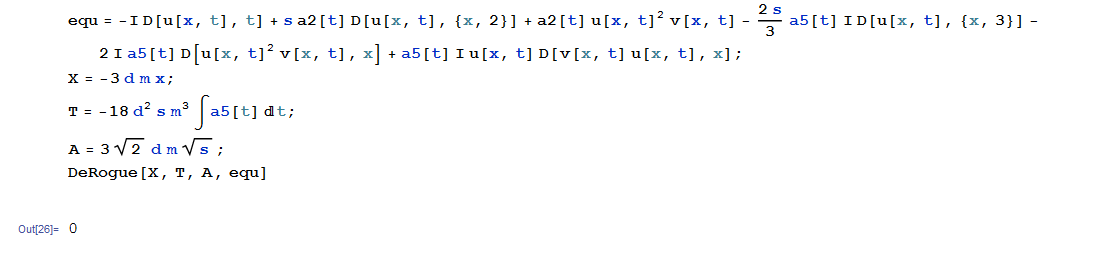
\includegraphics[width=\linewidth]{rogueResult.jpg}
	\caption{验证怪波运行结果}
	%with same parameters~$k=1 , \alpha_2(t)=1, \alpha_0(t)=0$.
	\label{}
\end{figure}
$X, T, A$ 是上一步变量变换得到的结果,$equ$ 是方程 (\ref{ss-1}) 的表达式,将变量变换后的怪波解代入 $equ$ 输出结果为零,完成验证。
\section{本章小结}
本章首先介绍了 Mathematica 内置 Wolfram 语言的基本语法、常用函数的用法与含义,然后用 Wolfram 封装了根据已知方程的怪波解得到另一方程的怪波解的过程。这个过程主要分为两个部分,第一,找到两个方程的变量变换的关系表达式,即 $DeReplace$ 函数的实现;第二,将变量变换的关系表达式代入已知的怪波解就可以得到另一方程的怪波解,并进行了验证,即 $DeRogue$ 函数的实现。最后,可以看到本章通过间接法得到的怪波解与第三章用 Darboux 变换法直接法求得的怪波解一致,变量变换为同一类型的方程的研究提供了捷径,也为求解怪波解提供了一个新思路。


